% Projeto de pesquisa (até 3 laudas), em LaTeX com a classe abnTeX2.
% COMPILAR COM XeLaTeX ou LuaLaTeX (no Overleaf: Menu > Compiler). Sequência: XeLaTeX > BibTeX > XeLaTeX > XeLaTeX.
% Arquivos: main.tex, referencias.bib e a pasta figuras/ (três imagens PNG).
% Observação: este código NÃO foi compilado por quem o escreveu (não havia LaTeX instalado). Confira o número de páginas.
\documentclass[11pt, a4paper, article, brazil]{abntex2}

% ---- Fonte: Arial (se não houver, usa TeX Gyre Heros, parecida) ----
\usepackage{fontspec}
\IfFontExistsTF{Arial}{\setmainfont{Arial}}{\setmainfont{TeX Gyre Heros}}

\usepackage{graphicx}
\usepackage{float}                         % figuras fixas no lugar (opção [H]), como no Word
\usepackage[brazilian, alf]{abntex2cite}   % citações autor-data (NBR 10520) e referências (NBR 6023)

\graphicspath{{figuras/}}
\setlength{\parindent}{1.25cm}             % recuo da primeira linha, como no Word
\OnehalfSpacing                            % espaçamento 1,5 no texto

\begin{document}

\begin{center}
  \textbf{Detecção de imagens geradas por IA em fotos políticas brasileiras}
\end{center}

\section{Resumo e justificativa}

Este projeto avalia se o UnivFD \cite{ojha2023} e o FSD \cite{nguyen2025}, detectores de imagens geradas por inteligência artificial, funcionam em fotografias de contexto político brasileiro. A contribuição é metodológica e empírica: estende a auditoria de vieses de bases de teste \cite{grommelt2024} a esse contexto e mede, com atalhos simples e pareamento por escore de propensão, quanto do desempenho aparente se deve a propriedades dos arquivos, e oferece um conjunto reproduzível de 1.027 imagens (513 reais de 50 políticos e 514 geradas, pareadas por cena). Nenhum detector discriminou real de gerada além do que atalhos simples explicam (AUC de 0,92 a 0,97).

A Justiça Eleitoral já exige rotulagem de conteúdo sintético em campanhas \cite{brasil2026}. Detectar que uma imagem é sintética, porém, não prova que ela seja enganosa, e um detector pode parecer acertar em uma base de teste apenas por pistas alheias à geração por IA, como o formato do arquivo \cite{grommelt2024}.

\section{Objetivos}

O objetivo geral é avaliar, de forma controlada, o desempenho do UnivFD e do FSD em fotos políticas brasileiras. Os objetivos específicos são:

\begin{alineas}
  \item identificar vieses nas bases de teste (formato, tamanho, nitidez);
  \item construir um conjunto reproduzível, pareado por cena, de fotos reais e geradas;
  \item medir o desempenho dos detectores com e sem a neutralização desses vieses, documentando o protocolo para reaplicação.
\end{alineas}

\section{Métodos}

O estudo teve quatro etapas. (1) Construção do conjunto: 513 fotos reais do Wikimedia Commons (licenças livres) e 514 imagens geradas por Stable Diffusion 1.5, SDXL \cite{podell2023} e SDXL-Turbo, a partir de legendas do BLIP \cite{li2022} de cada foto real, sem nomes e com pessoas fictícias (Figura~\ref{fig:exemplos}). (2) Padronização igual para as duas classes: recorte central de 512$\times$512 e JPEG de qualidade 90 (condição A) ou versão simulando rede social, 384$\times$384 e qualidade 75 (condição B). (3) Auditoria de atalhos: classificador simples sobre 11 medidas triviais, como tamanho do arquivo e nitidez. (4) Avaliação do UnivFD (limiar 0,5) e do FSD (limiar $-2{,}0$; 512 px) por AUC com intervalo de confiança de 95\% (reamostragem), no conjunto completo e em subconjunto pareado por escore de propensão \cite{rosenbaum1983}. Controles: sem JPEG adicional (condição C), dupla compressão nas falsas (condição D) e 513 recortes nativos dos originais do Commons.

\begin{figure}[H]
  \caption{Exemplos de foto real e de imagem gerada, um par por gerador}
  \label{fig:exemplos}
  \begin{center}
    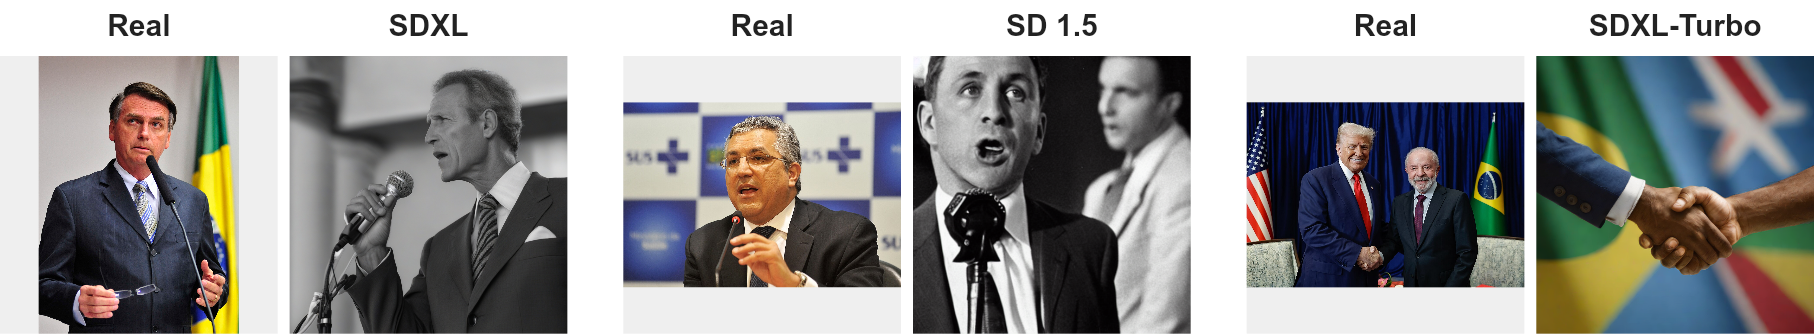
\includegraphics[width=\textwidth]{figura1_exemplos.png}
  \end{center}
  \fonte{Dados da pesquisa (2026). Fotos reais (Wikimedia Commons): G. Lima/Câmara dos Deputados (CC BY 3.0), E. Fiúza/ABr e R. Stuckert/PR/Agência Brasil (CC BY 3.0 BR).}
\end{figure}

\textbf{Participação da estudante e apoio recebido.} A estudante decidiu o desenho dos experimentos, executou-os e analisou e interpretou os resultados. A orientação contribuiu no refinamento e no direcionamento do tema. Um assistente de IA apoiou a escrita e a correção de erros de código e a organização dos textos; os resultados vêm de execuções feitas pela estudante.

\section{Resultados e conclusões}

Após padronizar tamanho, recorte e compressão, medidas simples separaram as classes com AUC de 0,946, como em outras bases \cite{grommelt2024}. Com os recortes nativos, a diferença de nitidez entre reais e falsas se inverteu, mas a separação seguiu alta (AUC de 0,92 a 0,96), como mostra a Figura~\ref{fig:atalhos}.

\begin{figure}[H]
  \caption{Nitidez mediana de reais e falsas (a) e AUC dos atalhos simples por condição (b)}
  \label{fig:atalhos}
  \begin{center}
    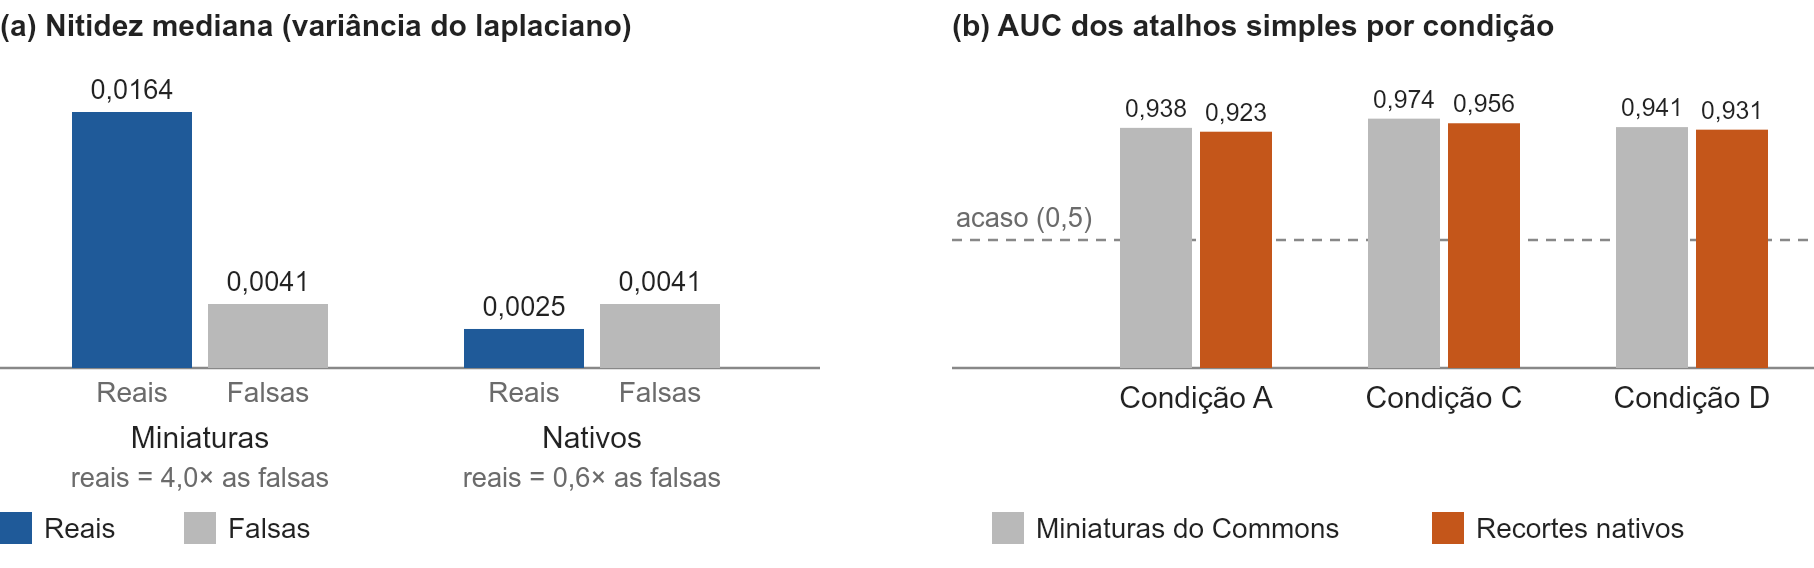
\includegraphics[width=\textwidth]{figura2_nitidez_atalhos.png}
  \end{center}
  \fonte{Dados da pesquisa (2026).}
\end{figure}

A Figura~\ref{fig:auc} mostra o AUC dos detectores. No conjunto completo, os dois ficaram abaixo de 0,5; no subconjunto pareado, o UnivFD ficou compatível com o acaso e o FSD, no acaso ou abaixo. A compressão JPEG não explicou o resultado.

\begin{figure}[H]
  \caption{AUC dos detectores, com intervalo de confiança de 95\% (0,5 = acaso)}
  \label{fig:auc}
  \begin{center}
    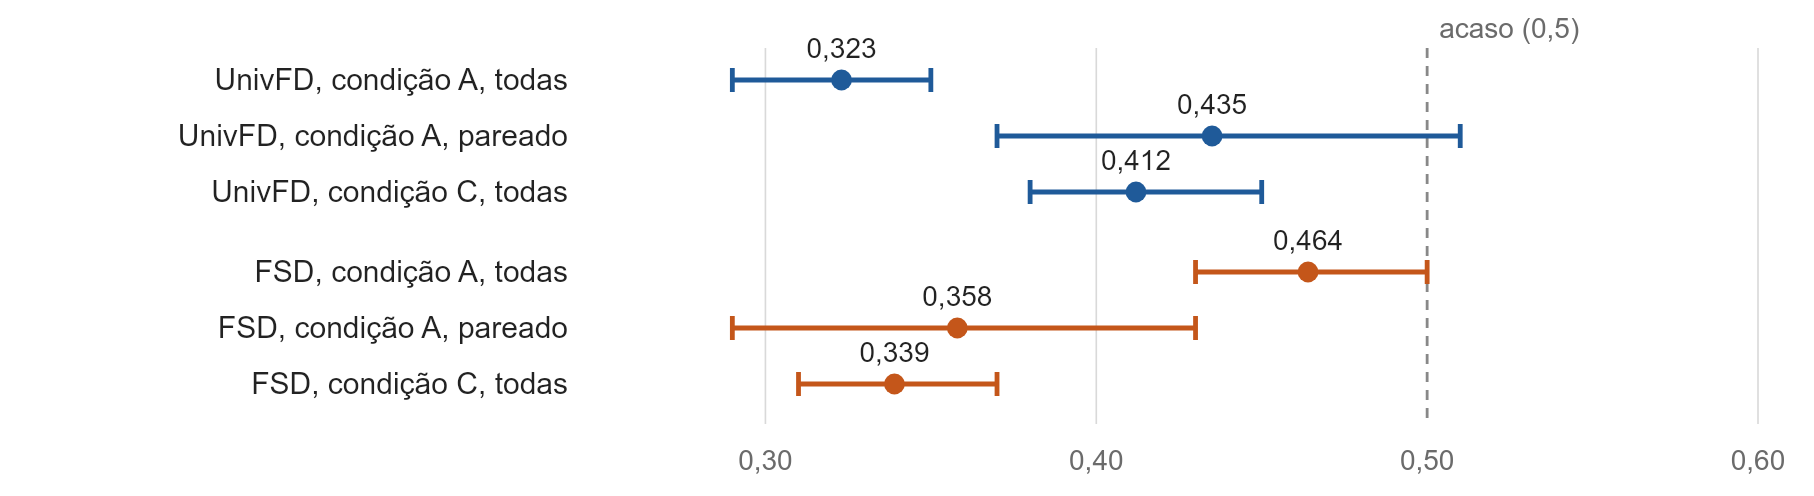
\includegraphics[width=\textwidth]{figura3_auc.png}
  \end{center}
  \fonte{Dados da pesquisa (2026).}
\end{figure}

Conclui-se que o desempenho aparente depende de propriedades dos arquivos, o que torna a auditoria de atalhos uma etapa necessária. As contribuições são: (i) um protocolo de auditoria de atalhos e pareamento; (ii) um conjunto reproduzível de fotos políticas brasileiras pareadas por cena; e (iii) a evidência de que, nas condições estudadas, UnivFD e FSD não discriminaram real de gerada além do que nitidez e tamanho explicam, o que não permite afirmar que falhem em geral, pois o FSD foi avaliado abaixo do tamanho padrão.

\bibliography{referencias}

\end{document}
